%% General definitions
\documentclass{article} %% Determines the general format.
\usepackage{a4wide} %% paper size: A4.
\usepackage[utf8]{inputenc} %% This file is written in UTF-8.
%% Some editors on Windows cannot save files in UTF-8.
%% If there is a problem with special characters not showing up
%% correctly, try switching "utf8" to "latin1" (ISO 8859-1).
\usepackage[T1]{fontenc} %% Format of the resulting PDF file.
\usepackage{fancyhdr} %% Package to create a header on each page.
\usepackage{lastpage} %% Used for "Page X of Y" in the header.
                      %% For this to work, you have to call pdflatex twice.
\usepackage{enumerate} %% Used to change the style of enumerations (see below).

\usepackage{amssymb} %% Definitions for math symbols.
\usepackage{amsmath} %% Definitions for math symbols.

\usepackage{tikz}  %% Pagacke to create graphics (graphs, automata, etc.)
\usetikzlibrary{automata} %% Tikz library to draw automata
\usetikzlibrary{arrows}   %% Tikz library for nicer arrow heads
\usetikzlibrary{positioning}    %% Tikz library for more positioning options

\usepackage{hyperref} %% hyperlinks

%% Left side of header
\lhead{\course\\\semester\\Exercise \homeworkNumber}
%% Right side of header
\rhead{\authorname\\Page \thepage\ of \pageref{LastPage}}
%% Height of header
\usepackage[headheight=36pt]{geometry}
%% Page style that uses the header
\pagestyle{fancy}

\newcommand{\authorname}{Benjamin Regez\\Luis Tritschler}
\newcommand{\semester}{Spring Semester 2026}
\newcommand{\course}{Foundations of Artificial Intelligence}
\newcommand{\homeworkNumber}{5}

\renewcommand{\thesection}{Exercise \homeworkNumber.\arabic{section}}


\begin{document}

\section{}
\begin{figure}[!ht]
    \centering
    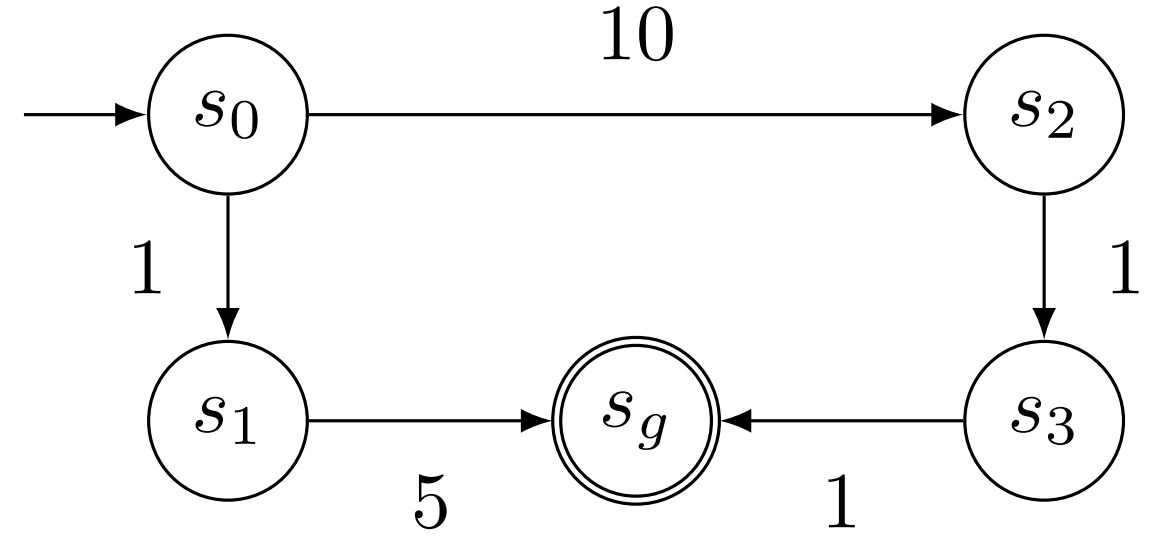
\includegraphics[width=0.4\linewidth]{assets/img_5_1.jpg}
    \label{fig:layout}
\end{figure}
\begin{enumerate}[(a)]
    \item greedy best-first search ($f(n) = h(n.\text{state})$):
    \begin{enumerate}[1.]
        \item expanding $s_0: open = \langle s_2(f=2), s_1(f=5) \rangle$, 
        $closed = \{ s_0(g=0) \}$
        \item expanding $s_2: open = \langle s_3(f=1), s_1(f=5) \rangle$,
        $closed = \{ s_0(g=0), s_2(g=10) \}$
        \item expanding $s_3: open = \langle s_g(f=0), s_1(f=5) \rangle$,
        $closed = \{ s_0(g=0), s_2(g=10), s_3(g=11) \}$
        \item expanding $s_g:$ found goal with cost 12
    \end{enumerate}
    \item A$^*$ $(f(n) = g(n) + h(n.state))$:
    \begin{enumerate}[1.]
        \item expanding $s_0: open = \langle s_1(f=6), s_2(f=12) \rangle$, 
        $closed = \{ s_0(g=0) \}$
        \item expanding $s_1: open = \langle s_g(f=6), s_2(f=12) \rangle$, 
        $closed = \{ s_0(g=0), s_1(g=1) \}$
        \item expanding $s_g:$ found goal with cost 6
     \end{enumerate}
\end{enumerate}


\section{}


\section{}


\section{}


\section*{Statement on scientific integrity}
% Google Translate was used to assist in translating individual words from
% German to English when writing down the exercise solutions.\\
% Apart from that, we solved the entire exercise sheet on our own.

\end{document}
